\documentclass[12pt]{article}
\usepackage[letterpaper, landscape, margin=0.5in]{geometry}
\usepackage{amsmath, amsthm, graphicx, tikz, pdflscape} 

\tikzset{
  treenode/.style = {shape=rectangle, %rounded corners,
                     draw, align=center,
                     top color=white, bottom color=blue!20},
  dec/.style = {shape=circle, rounded corners,
                    draw, align=center,
                    top color=white, bottom color=blue!20},
  last/.style = {shape=rectangle, %rounded corners,
                    draw, align=center,
                    top color=white, bottom color=green!20},
  root/.style     = {treenode, font=\Large, bottom color=red!30},
  env/.style      = {dec, font=\ttfamily\normalsize},
  end/.style = {last, font = \ttfamily\normalsize},
  dummy/.style    = {circle,draw}
}


\setlength\parindent{0pt}

\usepackage{fancyhdr}
\pagestyle{fancy}
\fancyhf{}
\lhead{Darshan Patel}
\rhead{Judgment and Decision Making}
\renewcommand{\footrulewidth}{0.4pt}
\cfoot{\thepage}

\begin{document}



$$ 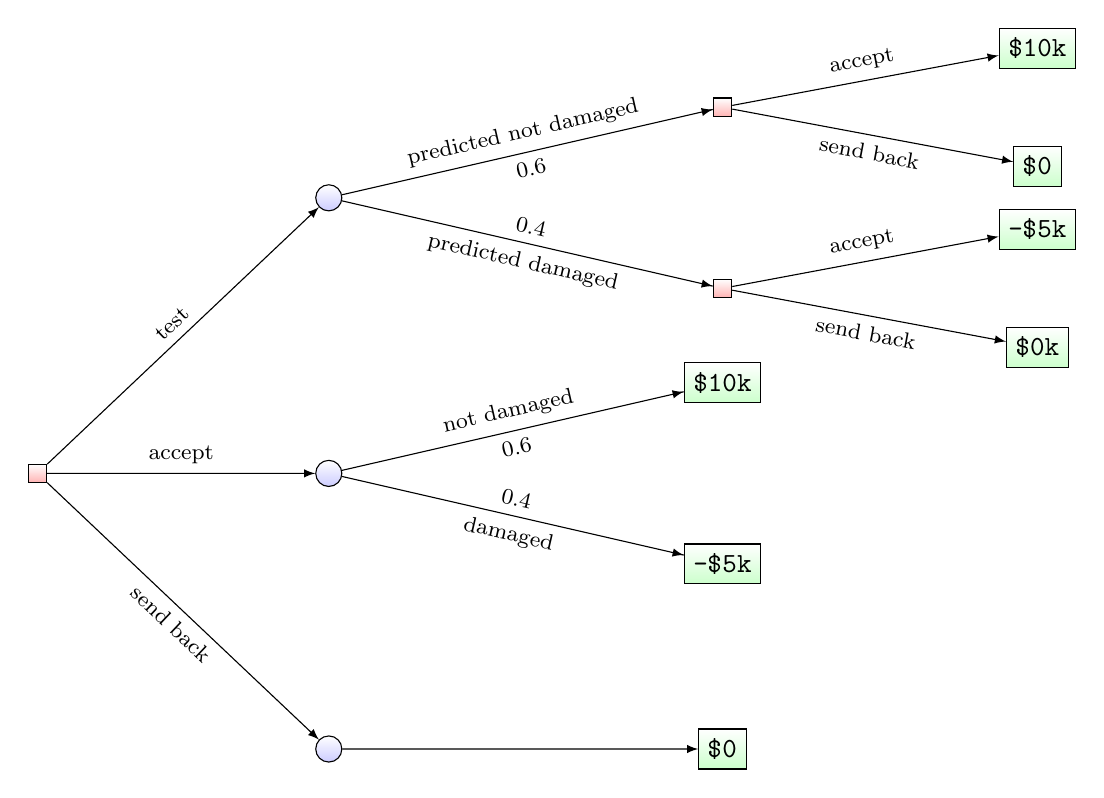
\begin{tikzpicture}
  [
  grow = right, 
  %sibling distance = 4cm,
 %level distance = 6cm,
  edge from parent/.style = {draw, -latex}, 
  every node/.style = {font = \footnotesize},
  sloped
  ]  
  
  \tikzstyle{level 1}=[sibling distance=35mm, level distance = 37mm] 
  \tikzstyle{level 2}=[sibling distance = 23mm, level distance = 50mm]
  \tikzstyle{level 3}=[sibling distance = 15mm, level distance = 40mm]
  %\tikzstyle{level 4}=[sibling distance = 12mm, level distance = 45mm]
  %\tikzstyle{level 5}=[sibling distance = 16mm, level distance = 50mm]


		
\node[root] {} 
	child{node [env] {}
		child{node [end] {\$0} }
	edge from parent node [below] {send back} }
	child{node [env] {}
		child{node [end] {-\$5k}
		edge from parent node [above] {0.4} 
		edge from parent node [below] {damaged} }
		child{node [end] {\$10k}
		edge from parent node [below] {0.6} 
		edge from parent node [above] {not damaged} }
	edge from parent node [above] {accept} }
	child{node [env] {}
		child{node [root] {}
			child{node [end] {\$0k}
			edge from parent node [below] {send back} }
			child{node [end] {-\$5k}
			edge from parent node [above] {accept} }
		edge from parent node [below] {predicted damaged} 
		edge from parent node [above] {0.4} }
		child{node [root] {}
			child{node [end] {\$0} 
			edge from parent node [below] {send back} } 
			child{node [end] {\$10k}
			edge from parent node [above] {accept} }
		edge from parent node [above] {predicted not damaged} 
		edge from parent node [below] {0.6} } 
	edge from parent node [above] {test} };
	
\end{tikzpicture} $$ \newpage

$$ 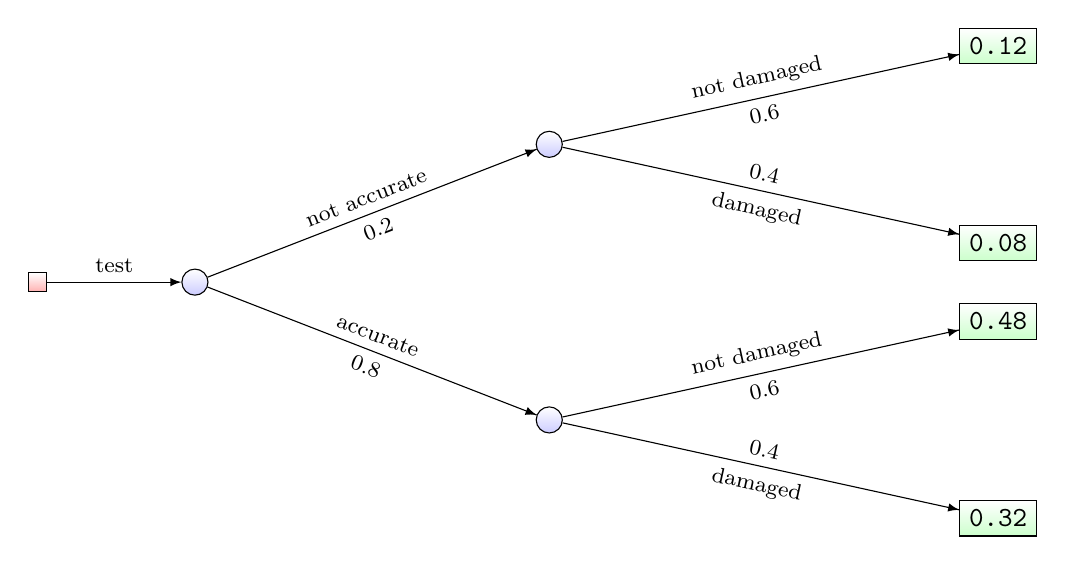
\begin{tikzpicture}[
  grow = right, 
  %sibling distance = 4cm,
 %level distance = 6cm,
  edge from parent/.style = {draw, -latex}, 
  every node/.style = {font = \footnotesize},
  sloped
  ]
  
   \tikzstyle{level 1}=[sibling distance=35mm, level distance = 20mm] 
  \tikzstyle{level 2}=[sibling distance = 35mm, level distance = 45mm]
  \tikzstyle{level 3}=[sibling distance = 25mm, level distance = 57mm]
    \tikzstyle{level 4}=[sibling distance = 25mm, level distance = 20mm]

	
\node[root]{}
	child{node [env] {}
		child{node [env] {}
			child{node [end] {0.32}
				%child{node [end] {-\$5k}}
			edge from parent node [below] {damaged} 
			edge from parent node [above] {0.4} }
			child{node [end] {0.48}
				%child{node [end] {\$10k} }
			edge from parent node [above] {not damaged}
			edge from parent node [below] {0.6} } 
		edge from parent node [above] {accurate}
		edge from parent node [below] {0.8} }
		child{node [env] {}
			child{node [end] {0.08}
				%child{node [end] {-\$5k} }
			edge from parent node [below] {damaged} 
			edge from parent node [above] {0.4} }
			child{node [end] {0.12}
				%child{node [end] {\$10k}}
			edge from parent node [above] {not damaged}
			edge from parent node [below] {0.6} } 
		edge from parent node [above] {not accurate}
		edge from parent node [below] {0.2} }
	edge from parent node [above] {test} };	
			
\end{tikzpicture} $$ 

\newpage


$$ 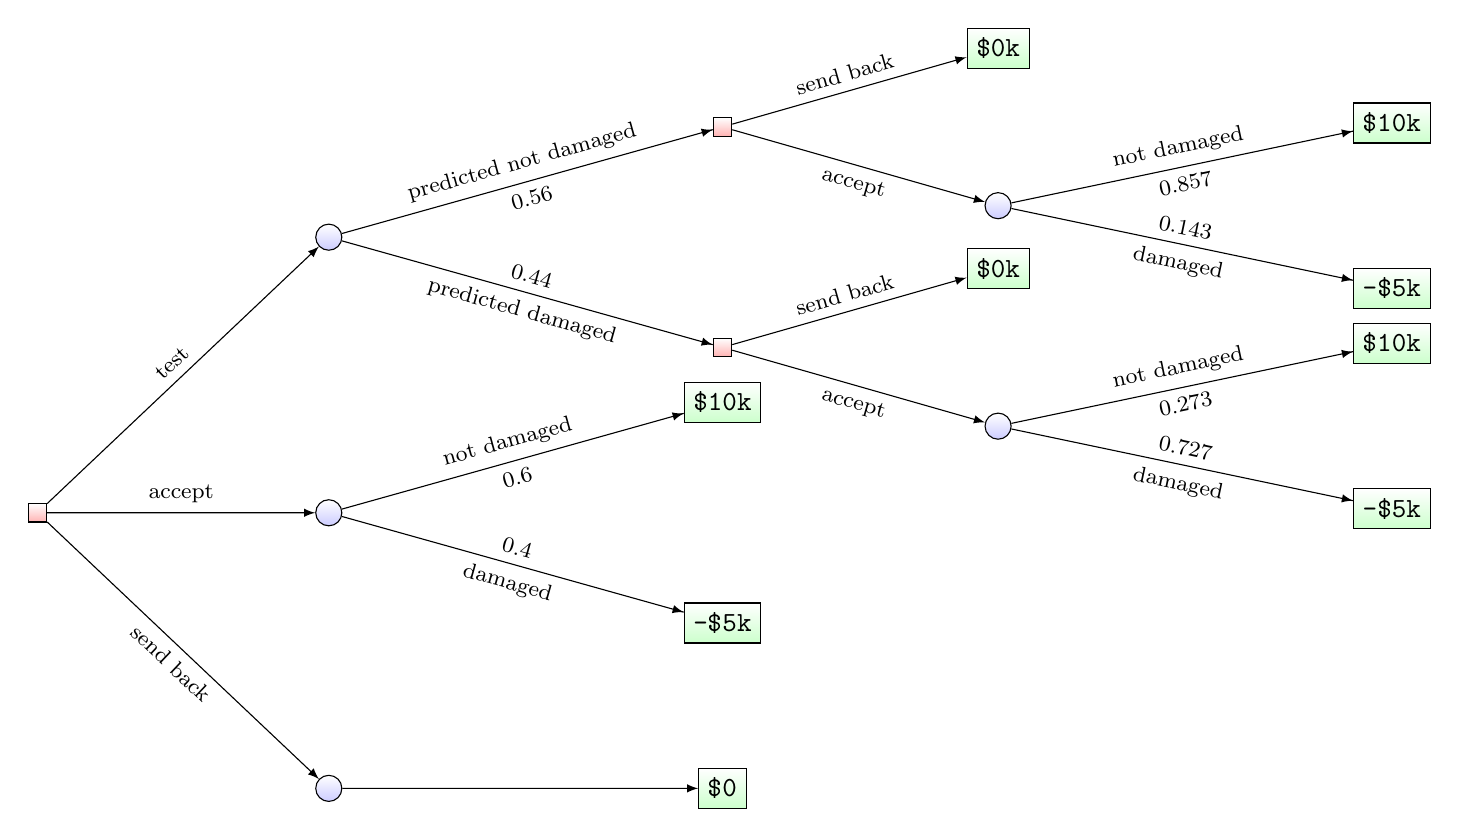
\begin{tikzpicture}
  [
  grow = right, 
  %sibling distance = 4cm,
 %level distance = 6cm,
  edge from parent/.style = {draw, -latex}, 
  every node/.style = {font = \footnotesize},
  sloped
  ]  
  
  \tikzstyle{level 1}=[sibling distance=35mm, level distance = 37mm] 
  \tikzstyle{level 2}=[sibling distance = 28mm, level distance = 50mm]
  \tikzstyle{level 3}=[sibling distance = 20mm, level distance = 35mm]
  \tikzstyle{level 4}=[sibling distance = 21mm, level distance = 50mm]
  %\tikzstyle{level 5}=[sibling distance = 16mm, level distance = 50mm]


		
\node[root] {} 
	child{node [env] {}
		child{node [end] {\$0} }
	edge from parent node [below] {send back} }
	child{node [env] {}
		child{node [end] {\text{-}\$5k}
		edge from parent node [above] {0.4} 
		edge from parent node [below] {damaged} }
		child{node [end] {\$10k}
		edge from parent node [below] {0.6} 
		edge from parent node [above] {not damaged} }
	edge from parent node [above] {accept} }
	child{node [env] {}
		child{node [root] {}
			child{node [env] {}
				child{node [end] {\text{-}\$5k} 
				edge from parent node [below] {damaged}
				edge from parent node [above] {0.727} }
				child{node [end] {\$10k}
				edge from parent node [above] {not damaged}
				edge from parent node [below] {0.273} }
			edge from parent node [below] {accept} }
			child{node [end] {\$0k}
			edge from parent node [above] {send back} }
		edge from parent node [below] {predicted damaged} 
		edge from parent node [above] {0.44} }
		child{node [root] {}
			child{node [env] {}
				child{node [end] {\text{-}\$5k} 
				edge from parent node [below] {damaged}
				edge from parent node [above] {0.143} }
				child{node [end] {\$10k}
				edge from parent node [above] {not damaged}
				edge from parent node [below] {0.857} }
			edge from parent node [below] {accept} }
			child{node [end] {\$0k}
			edge from parent node [above] {send back} }
		edge from parent node [above] {predicted not damaged}
		edge from parent node [below] {0.56} } 
	edge from parent node [above] {test} };
	
\end{tikzpicture} $$



\end{document}			
			
			
			
			
			
			
